\begin{opgavetekst}{Problem 1}
\end{opgavetekst}
\begin{delopgave}{1}
	Find the derivative of the following functions
	\begin{align*}
		&1) \   x^2\cos(x)   &&2) \  e^x\cdot\frac{1}{x}     \\
		&3) \ \sqrt{x}\ln(x) &&4) \ \sin(x)\cos(x)  \\
	\end{align*}
\end{delopgave}

\begin{opgavetekst}{Problem 2}
\end{opgavetekst}
\begin{delopgave}{1}
	Find the derivative of the following functions
	\begin{align*}
		&1) \  e^{-5x+10}   &&2) \  4\ln(x^2-10x+7)     \\
		&3) \ \frac{0.7}{\cos(x)} &&4) \ 7\sin\left(\frac{1}{x}\right)  \\
	\end{align*}
\end{delopgave}

\begin{opgavetekst}{Problem 3}
\end{opgavetekst}
\begin{delopgave}{1}
	Find the derivative of the following functions
	\begin{align*}
		&1) \  \frac{x^2+5}{x-10}   &&2) \  \frac{\cos(x)}{\sin(x)}     \\
		&3) \ \frac{\ln(x)}{4x^2 + 7x - 10} &&4) \ \frac{\sqrt{x}}{e^x}  \\
	\end{align*}
\end{delopgave}


\begin{opgavetekst}{Problem 4}
\end{opgavetekst}
\begin{delopgave}{1}
	Find the derivative of the following functions
	\begin{align*}
		&1) \  \sqrt{x^2-10x}\cdot\ln(x)   &&2) \  \cos\left(\ln(x)\cdot x^4\right)   \\
	\end{align*}
\end{delopgave}

\begin{opgavetekst}{Problem 4}	
	A function $f$ is given by
	\begin{align*}
		f(x) = x^4\cdot\ln(x), \ x> 0.
	\end{align*}
\end{opgavetekst}
\begin{delopgave}{1}
	Determine the value of $\frac{df}{dx}$ at $x = 1$.
\end{delopgave}

\begin{opgavetekst}{Problem 5}
	A function $g$ is given by
	\begin{align*}
		g(x) = \sqrt{x^2-3x}.
	\end{align*}
\end{opgavetekst}
\begin{delopgave}{1}
	Determine an equation for the normal line to the graph of $g$ in the point $(4,g(4))$.
\end{delopgave}

\begin{opgavetekst}{Problem 6}
	A function $h$ is given by
	\begin{align*}
		h(x) = \frac{1}{4}x^4-\frac{2}{3}x^3-\frac{3}{2}x^2 + \sqrt{0.9}
	\end{align*}
\end{opgavetekst}
\begin{delopgave}{1}
	Determine all the stationary points for $h$ and denote the type of stationary point. 
\end{delopgave}

\begin{opgavetekst}{Problem 7}
A container for ice-cream should be shaped as seen in Figure \ref{fig:pindeis}. It should consist of a buttom, a domed top and a cylinder for sides. The volume of the container should be 150ml (150cm$^3$).
	\begin{figure}[H]
	\centering
	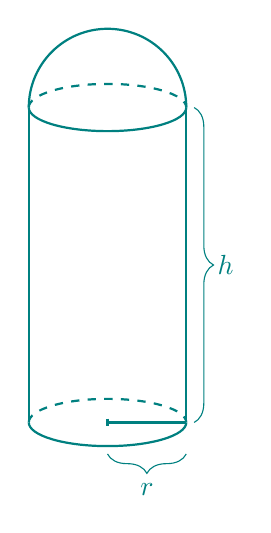
\begin{tikzpicture}  
		%Sides
		\draw[color = teal, thick] (0,0) -- (0,4);
		\draw[color = teal, thick] (2,0) -- (2,4);
		%Buttom and top
		\draw[color = teal, thick] (0,0) arc [start angle = 180, end angle = 360,
		 x radius = 1cm, y radius = 0.3cm];
		\draw[color = teal, thick, dashed] (0,0) arc [start angle = 180, end angle = 0,
		 x radius = 1cm, y radius = 0.3cm]; 
		 \draw[color = teal, thick] (0,4) arc [start angle = 180, end angle = 360,
		 x radius = 1cm, y radius = 0.3cm];
		\draw[color = teal, thick, dashed] (0,4) arc [start angle = 180, end angle = 0,
		 x radius = 1cm, y radius = 0.3cm]; 
		 %Half-ball
		 \draw[color = teal, thick] (0,4) arc [start angle = 180, end angle = 0, radius = 1cm];
		 %Braces
		 \draw[decorate,decoration = {brace,amplitude = 7pt, mirror},color = teal] (2.1,0) -- (2.1,4);
		 \node[color = teal] at (2.5,2) {$h$};
		 \draw[decorate,decoration = {brace,amplitude = 7pt, mirror},color = teal] (1,-0.4) -- (2,-0.4);
		 \node[color = teal] at (1.5,-0.85) {$r$};
		 \draw[color = teal, thick] (2,0) -- (1,0);
		 \draw[color = teal, thick] (1,0.05) -- (1,-0.05);
	\end{tikzpicture}
	\caption{Container}
	\label{fig:pindeis}
\end{figure}
\phantom{h}
\end{opgavetekst}	
\begin{delopgave}{1}
	Determine the dimensions of the container such that the surface area of the container is minimised. 
	You must show your work, and you can use your GDC to minimise your area function.
\end{delopgave}